


\documentclass{beamer}
\usetheme{ucl}

\usepackage[utf8]{inputenc}


%%% Increase the height of the banner: the argument is a scale factor >=1.0
%\setbeamertemplate{banner}[ucl][10.0]

%%% Change the colour of the main banner
%%% The background should be one of the UCL colours (except pink or white):
%%%   black,darkpurple,darkred,darkblue,darkgreen,darkbrown,richred,midred,
%%%   navyblue,midgreen,darkgrey,orange,brightblue,brightgreen,lightgrey,
%%%   lightpurple,yellow,lightblue,lightgreen,stone
\setbeamercolor{banner}{bg=darkpurple}
%\setbeamercolor{banner}{bg=yellow,fg=black}

%%% Add a stripe behind the banner
%\setbeamercolor{banner stripe}{bg=darkpurple,fg=black}

%%% The main structural elements
\setbeamercolor{structure}{fg=black}

%%% Author/Title/Date and slide number in the footline
\setbeamertemplate{footline}[author title date]

%%% Puts the section/subsection in the headline
% \setbeamertemplate{headline}[section]

%%% Puts a navigation bar on top of the banner
%%% For this to work correctly, the each \section command needs to be
%%% followed by a \subsection. Requires one extra compile.
% \setbeamertemplate{headline}[miniframes]
%%% Accepts an optional argument determining the width
% \setbeamertemplate{headline}[miniframes][0.3\paperwidth]


%%% Puts the frame title in the banner
%%% Won't work correctly with the above headline templates
%\useoutertheme{ucltitlebanner}
%%% Similar to above, but smaller (and puts subtitle on same line as title)
\useoutertheme[small]{ucltitlebanner}

%%% Gives block elements (theorems, examples) a border
% \useinnertheme{blockborder}
%%% Sets the body of block elements to be clear
% \setbeamercolor{block body}{bg=white,fg=black}

%%% Include CSML logo on title slide
%\titlegraphic{\includegraphics[width=0.16\paperwidth]{csml_logo}}

%%% Include CSML logo in bottom right corner of all slides
%\logo{\includegraphics[width=0.12\paperwidth]{csml_logo}}

%%% Set a background colour
% \setbeamercolor{background canvas}{bg=lightgrey}

%%% Set a background image
%%% Some sample images are available from the UCL image store:
%%%   https://www.imagestore.ucl.ac.uk/home/start
% \setbeamertemplate{background canvas}{%
%   \includegraphics[width=\paperwidth]{imagename}}



%%%%%% Some other settings that can make things look nicer
%%% Set a smaller indent for description environment
\setbeamersize{description width=2em}
%%% Remove nav symbols (and shift any logo down to corner)
\setbeamertemplate{navigation symbols}{\vspace{-2ex}}








\DeclareMathOperator{\Cov}{Cov}
\DeclareMathOperator{\Var}{Var}
\DeclareMathOperator{\E}{\mathbb{E}}
\DeclareMathOperator{\Proba}{\mathbb{P}}

\newcommand{\Covb}[2]{\ensuremath{\Cov\!\left[#1,#2\right]}}
\newcommand{\Eb}[1]{\ensuremath{\E\!\left[#1\right]}}
\newcommand{\Pb}[1]{\ensuremath{\Proba\!\left[#1\right]}}
\newcommand{\Varb}[1]{\ensuremath{\Var\!\left[#1\right]}}

% norm
\newcommand{\norm}[1]{\| #1 \|}

\newcommand{\indep}{\rotatebox[origin=c]{90}{$\models$}}





\usepackage{newtxmath,amsmath,amssymb,graphicx,bibentry,bbm,ragged2e}
\usepackage[english]{babel}

\makeatletter

\newcommand{\noun}[1]{\textsc{#1}}
\newcommand{\jitem}[1]{\item \begin{justify} #1 \end{justify} \vfill{}}
\newcommand{\sframe}[2]{\frame{\frametitle{#1} #2}}

\newenvironment{centercolumns}{\begin{columns}[c]}{\end{columns}}
%\newenvironment{jitem}{\begin{justify}\begin{itemize}}{\end{itemize}\end{justify}}



%\usetheme{Warsaw}
%\setbeamertemplate{footline}[text line]{}
%\setbeamertemplate{headline}{}
%\setbeamercolor{structure}{fg=purple!50!blue, bg=purple!50!blue}

%\setbeamersize{text margin left=15pt,text margin right=15pt}

%\setbeamercovered{transparent}


\@ifundefined{showcaptionsetup}{}{%
 \PassOptionsToPackage{caption=false}{subfig}}
\usepackage{subfig}

\usepackage[utf8]{inputenc}
\usepackage[T1]{fontenc}

\usepackage{multirow}


\makeatother

\def \draft {1}

\usepackage{xparse}
\usepackage{ifthen}
\DeclareDocumentCommand{\comment}{m o o o o}
{\ifthenelse{\draft=1}{
    \textcolor{red}{\textbf{C : }#1}
    \IfValueT{#2}{\textcolor{blue}{\textbf{A1 : }#2}}
    \IfValueT{#3}{\textcolor{ForestGreen}{\textbf{A2 : }#3}}
    \IfValueT{#4}{\textcolor{red!50!blue}{\textbf{A3 : }#4}}
    \IfValueT{#5}{\textcolor{Aquamarine}{\textbf{A4 : }#5}}
 }{}
}
\newcommand{\todo}[1]{
\ifthenelse{\draft=1}{\textcolor{red!50!blue}{\textbf{TODO : \textit{#1}}}}{}
}




\begin{document}


\title[ABM for infectious disease policies]{Exploring and optimising infectious disease policies with a stylised agent-based model}

\author[Kang and Raimbault]{Jeonghwa Kang$^1$ and Juste Raimbault$^{2,1,\ast}$\\\medskip
$^{\ast}$\texttt{juste.raimbault@ign.fr}
}

\institute[UCL]{$^{1}$Center for Advanced Spatial Analysis, University College London\\
$^{2}$LASTIG, Univ. Gustave Eiffel, IGN-ENSG
}


\date[31/05/2023]{FRCCS 2023\\
Session O4: Diffusion \& Epidemics\\
May 31st 2023
}

\frame{\maketitle}

% The quantitative study of the spread of infectious diseases is a crucial aspect to design health policies and foster responsiveness, as the recent COVID-19 pandemic showed at an unprecedented scale. In-between abstract theoretical models and large-scale data driven microsimulation models lie a broad set of modelling tools, which may suffer from various issues such as parameter uncertainties or the lack of data. We introduce in this paper a stylised ABM for infectious disease spreading, based on the SIRV compartmental model. We account for a certain level of geographical detail, including commuting modes and workplaces. We apply to it a set of model validation methods, including global sensitivity analysis, surrogates, and multi-objective optimisation. This shows how such methods could be a new tool for more robust design and optimisation of infectious disease policies.


\section{Introduction}


\sframe{Complexity of infectious disease policies}{

%The impact of one of the fatal epidemics in history, the Black Death, has led to the death of almost one-third of the population of Europe, and the most recent epidemic in the world today, COVID-19, is currently costing millions of valuable human lives \cite{glatter2021history}. Before the introduction of mathematical and computational modelling, humans had little knowledge of effectively controlling and minimising the spread of infectious diseases. Furthermore, the importance of forecasting the spread of diseases in recent years has become even more crucial as the world is rapidly globalising and becoming closer with ever-advancing technologies that make it easier for humans to travel faster and further around the globe \cite{saker2004globalization}. Beyond the health disease of epidemics, many dimensions of social systems are affected, with for example broad economic impacts \cite{boucekkine2021economics}. The current world is a highly complex systems in which various factors will play a role in decision-making \cite{bickley2021does}. Designing disease control strategies imply accounting for various interacting factors and finding a compromise between multiple objectives \cite{kaszowska2022immunity}.
%The first modelling approach to disease spreading was in the 17th century as John Graunt  conducted an empirical study on infections affecting individuals in various regions in Britain \cite{morabia2013epidemiology}. Bernouilli introduced in the 18th century an equation-based approach to studying the outbreak of the smallpox epidemic in Europe \cite{dietz2002daniel}. Most recent modelling approaches range from elaborated mathematical models to data-driven microsimulation models. The recent pandemic has shown the usefulness of quantitative modelling to evaluate policies, such as how to vaccinate the population \cite{bosetti2022epidemiology} or to evaluate which degree of lockdown is necessary.
%Agent-based modelling are proposed by some researchers as a powerful tool to explore practical scenarios for decision-making when managing the spread of infectious diseases \cite{miksch2019should}. The classical epidemiological modelling relies on compartmental models, such as the SIR model (Susceptible, Infected, Recovered), with differential equations governing the evolution of the different compartments, or in some cases discrete-time equations \cite{ramani2004oscillating}. More recent extensions, such as the SEIRD model \cite{chowell2008seasonal}, include a more detailed description of states. \cite{chumachenko2018agent} describe an agent-based model based on similar states for agents. The advantage of the ABM approach is that one can define agent characteristics such as location, age, and many other factors believed necessary in the model for each agent. Once the agents are defined with their own set of characteristics, they proceed through a set of rules which enable them to interact with other groups of agents within the simulation. Age groups have contact probabilities to simulate the interactions and infections between agents. More details can be included in an ABMM, such as wearing face masks or respecting social distancing \cite{minoza2021covid}. Furthermore, the infectious disease may interact with other chronic conditions, what can be accounted for in an ABM \cite{fekadu2021impact}.

\bigskip

\textit{Complexity of multi-objective decision making for epidemics and pandemics in a globalised world \cite{saker2004globalization} \cite{bickley2021does}}

\bigskip
\bigskip
\bigskip

$\rightarrow$ current models for decision-making range from mathematical models \cite{brauer2008compartmental} to data-driven simulation models \cite{buczak2012data}

\bigskip

$\rightarrow$ agent-based modelling as a flexible and generic modelling tool particularly suited for decision-making \cite{miksch2019should} \cite{minoza2021covid}


}



\sframe{Research question}{

% We propose in this paper to explore the potential of agent-based modeling to design and optimise epidemiological policies. We introduce a stylised model for the spread of infectious diseases, which is hybrid in the sense that it lies halfway large data-driven models and abstract theoretical models. We account for geographical factors, in particular commuting and workplaces. We focus, as an illustration, for two policy factors, which are social distancing and face masks \cite{kwon2021association}, and vaccination \cite{bicher2022model}. Our main contribution is the application of state-of-the-art model sensitivity analysis and validation techniques \cite{raimbault2019methods} to such a stylised model, opening research perspectives to cases where data is lacking, model parametrisation is uncertain, or actors have not the ressources to implement a large scale model, but where accounting for spatial and social structure remains crucial.
% A few examples of the application of such techniques to epidemiological models can be found in the literature. \cite{baquela2022optimising} utilise a multi-objective optimisation algorithm for the distribution of limited vaccines resources. \cite{wu2013sensitivity} review sensitivity analysis of infectious disease models. No systematic application of an umbrella of model validation methods can however be found.

\bigskip

$\rightarrow$ validation, exploration and sensitivity analysis of ABMs and other approaches not frequent in the literature \cite{baquela2022optimising}\cite{wu2013sensitivity}

\medskip

$\rightarrow$ how can extensive model validation techniques be used for stylised models?

\bigskip
\bigskip

\textbf{Research question}

\medskip

\textit{We build a stylised ABM for the spread of infectious disease which focuses on masking and vaccination and apply model validation methods, to investigate if lack of data and uncertainty can be compensated for through model validation.}



}

\section{Simulation model}

\sframe{Stylised simulation model}{

% Our simulation model projects a real-life situation where agents commute from home to their designated workplaces via different modes of transportation on a fixed daily schedule. At the beginning of the simulation, the entire population is set to susceptible. Then, an infected agent is introduced daily for the first 30 days because if none of the infected agents gets introduced into the environment, the infection process does not happen. The model's output parameters include the number of agents associated within each state of the compartmental model upon which the ABM is based.
% The main interest of this research is investigating the effectiveness of various pre-defined model input parameters on spreading and controlling infectious diseases that result while the agents are commuting from home to the workplace. This model assumes that most human interactions occur while people travel and work. Hence, the scenario is primarily about people commuting from home to their designated workplaces via different modes of transportation, closely depicting ordinary people's daily routine. The simulation of this model considers several essential assumptions. The entire duration of the simulation is set to 365 days. Each day is equivalent to 24 ticks. Hence, each tick is equivalent to an hour. A single day comprises three pre-defined phases: the 'Home-hour', 'Commute-hour and 'Work-hour' phases, as show in Fig.~\ref{fig:modeltrans}.
% During these phases, the movement of agents is completely randomised. No learning behaviour alternates the agents' movement in the simulation since it would be difficult for an individual to be fully aware of another agent’s infection status. During the interaction, agents fall into one of the four states defined by the SIRV compartmental model, which this research’s ABM is based upon. The SIRV model is an extended SIR model that accounts for the vaccination of the susceptible population \cite{poonia2022enhanced}. The agent states are shown in Fig.~\ref{fig:agentstates}.
% Agents can interact with each other based on the state in which they fall. However, the interaction and infection processes are set to occur between the agents within the same patch only. The infection does not happen during the 'Home-hour' phase as this model does not consider social activities or household infections. During the 'Commute-hour' phase, an infected agent can only infect the susceptible agents that use the same mode of transportation as itself. It would be logically sensible that an infected agent commuting via train can only interact with and infect other susceptible agents commuting via the same mode of transportation. This same logic applies during the 'Work-hour' phase, where an infected agent can only interact with and infect other susceptible agents working in the same company. We include four modes of transportation in the model (metro, train, walking, car), and consider stylised company size distributions (7 large companies, 4 medium sized, 4 small). There are total of fifteen companies which are randomly categorised into small, mid, and big-sized companies. The central assumption is that the bigger the company size, the more the human interactions involved. Hence, the agents working in a big-sized companies are more likely to get infected than the agents working in mid and small-sized companies.
%At the beginning of the simulation, 1500 susceptible agents are randomly distributed in the simulation environment. The variable values for the agents, such as the transportation and company, are randomly assigned during the setup stage. An infected agent is then constantly introduced at a random location for the simulation's first month (30 days). Every day, a random percentage value from zero to one percent of the total population gets replaced. This is based on the assumption that the population is dynamic. A certain number of people leave the area, and others come to stay in the area. Hence, the total population is not fixed to the initial population throughout the simulation.

\begin{itemize}
	\item Realistic geographical context, with commuting of workers simulated through the day (1h tick) for 365 days
	\item Simple SIRV agent dynamics within places (public transport and workplace)
	\item 4 transportation modes and a stylised setup for company sizes
	\item $N=1500$ agents randomly assigned, with less than 1\% daily renewed (open world)
\end{itemize}

}

\sframe{Agent states}{

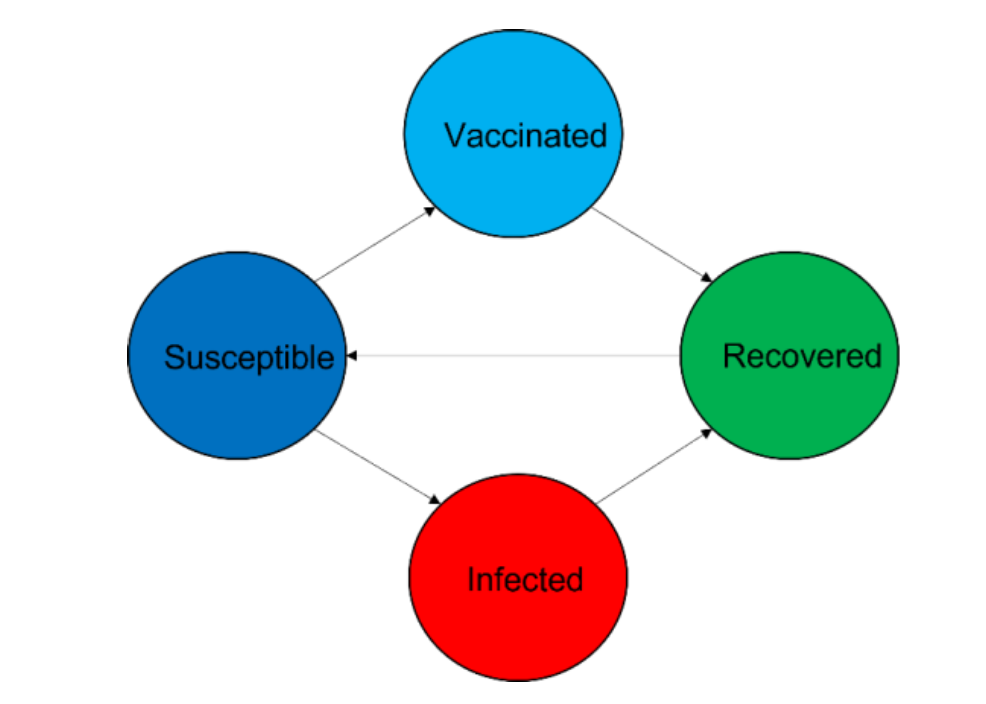
\includegraphics[width=0.46\linewidth]{../figures/AgentStates.png}
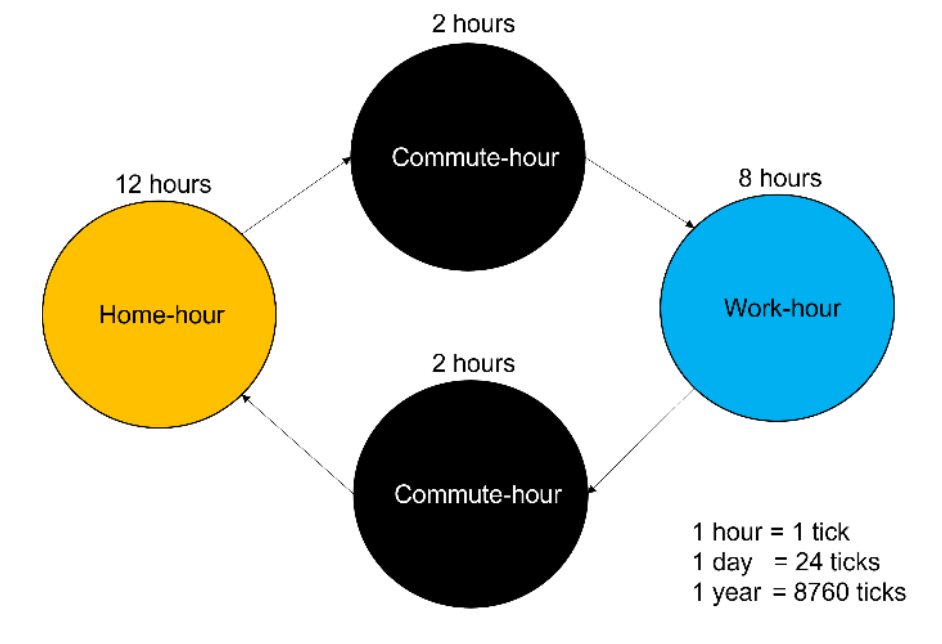
\includegraphics[width=0.46\linewidth]{../figures/ModelTransitions.png}

(Left) agent states; (Right) daily cycle.

}

\sframe{Model dynamics}{

\centering
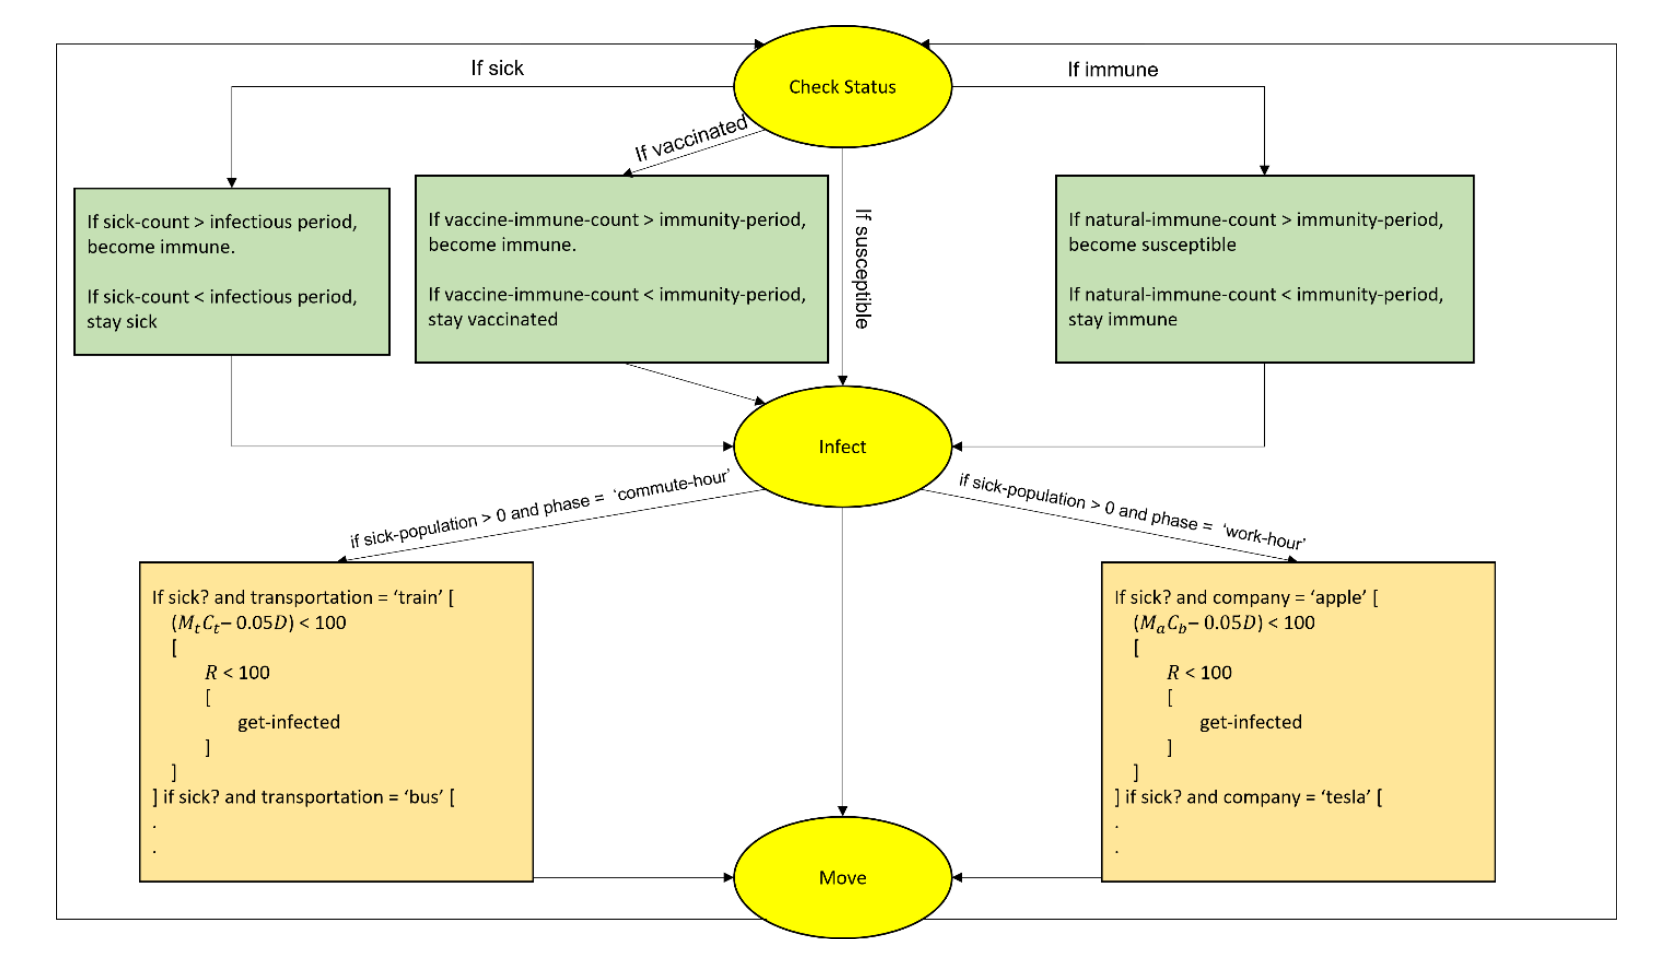
\includegraphics[width=0.9\linewidth]{../figures/modelDynamics.png}

}

\sframe{Model setup}{

% We give in this section more details on the parametrisation of the stylised model.
% \subsubsection{Global variables}
%Infection rates are calculated based on the values of the global, patch and turtle variables. The variables that define contact rates for each mode of transportation and company are pre-defined with specific values.
%For transportation contact rates, we take stylised values decreasing with the density one can expect in each transport mode: $c_{bus} = 40\%$, $c_{metro} = 35\%$, $c_{train} = 30\%$, $c_{walk} = 10\%$, $c_{car} = 10\%$.
%No discrete values define the accurate contact rates for different modes of transportation, but the general assumption was made based on the understanding that the lower the capacity of transportation, the higher the density; hence, the higher contact rates between the passengers. The contact rate specifically for the car is set to zero because it is assumed that an agent who commutes by a car makes no contact with other agents during the 'Commute- hour' phase. The same logic was applied when defining the contact rates for different companies. The assumption was based on the understanding that the bigger the company size, the more the agents interact.
%For contact rates on work site, we therefore take the following values: $c_{Big} = 40\%$, $c_{Medium} = 35\%$, $c_{Small} = 30\%$
%\subsubsection{Agent variables}
%The importance of wearing a mask while interacting with an infected agent can significantly reduce the chance of infection. Furthermore, patients with cardiovascular diseases are known to be at high risk of getting an infection \cite{ielapi2020cardiovascular}. Due to these reasons, we have pre-defined values for infection risk rates based on the combination of these two variables: No mask \& Cardio = 50\% risk rate; Mask \& Cardio = 45\%; No mask \& Cardio = 15\%; Mask \& No Cardio = 10\%.

\textbf{Global variables: } stylised contact rates for transport $c_{bus} = 40\%$, $c_{metro} = 35\%$, $c_{train} = 30\%$, $c_{walk} = 10\%$, $c_{car} = 10\%$ and companies $c_{Big} = 40\%$, $c_{Medium} = 35\%$, $c_{Small} = 30\%$

\bigskip
\bigskip

\textbf{Agent variables: } higher infection rate for cardio-vascular sick individuals \cite{ielapi2020cardiovascular}

$\rightarrow$ predefined infection risk rates depending on agent characteristics: No mask \& Cardio = 50\% risk rate; Mask \& Cardio = 45\%; No mask \& Cardio = 15\%; Mask \& No Cardio = 10\%


}

\sframe{Model parameters and indicators}{

\textbf{Model parameters explored:}

\begin{itemize}
	\item Infectious period (2-4 weeks)
	\item Immunity period (9-11 months)
	\item Vaccination rate
	\item Social distancing level (3 levels, each reducing contact rate by 5\%)
\end{itemize}

\bigskip

\textbf{Model indicators: } agents in each state, cumulated infections and vaccinations.

%As mentioned previously, the ABM is constructed under the concept of the SIRV compartmental model. Therefore, the indicators consist of proportional numbers of agents in each compartment, including susceptible, infected, recovered, and vaccinated.


}



\section{Results}

\sframe{Model implementation and exploration}{

%The model is implemented in NetLogo, which is a reasonable choice for such hybrid models in which visualisation is important. It is integrated into the OpenMOLE platform for model exploration \cite{reuillon2013openmole} to carry out the numerical experiments described below. Source code of the model and exploration scripts are openly available on a git repository at \texttt{}.
%The pre-defined input parameter values of the model are the following: infectious-period $\in \{ 2, 3, 4 )\}$ (weeks); immunity-period $\in \{ 4, 5, 6  )\}$ (months); vaccination-rate $\in \{ 0, 0.25, 0.5 \}$ (\%); social-distancing-levels $\in \{1, 2, 3\}$ (levels).
%This results in 81 different combinations of the input parameter values for a grid sampling. The model is set to run over 125 times for every combination of the input parameter values, and the output parameters’ average values are obtained at the end.

$\rightarrow$ model implemented in NetLogo (role of visualisation and interactivity in the model construction process)

\bigskip

$\rightarrow$ embedded into the OpenMOLE platform for model exploration and validation \cite{reuillon2013openmole}

\begin{center}
	
\includegraphics[height=0.1\textheight]{iconOM}
	
\includegraphics[height=0.1\textheight]{openmole}
\end{center}

$\rightarrow$ 4 dimensions parameter space explored through numerical experiments

}

\sframe{Statistical behavior}{

%The LHS (Latin hypercube Sampling) method was used to explore the input space of the model. A total of 10,000 samples were drawn during the process (corresponding to 4 days and 4h of CPU time for model execution), used to study statistical properties of model indicators.
%The histograms in Fig.~\ref{fig:histograms} illustrate the four different output indicators of the model. The histograms in the upper row comprise the ‘ProportionSick’ and the ‘ProportionImmune’ histograms, which appear symmetrical, but the skewness values indicate the traits of negative skewness on each histogram plot. Both kurtosis values are negative, suggesting that the distributions are thin-tailed. From this finding, we can assume that they generally follow characteristics of the platykurtic distribution. The ‘ProportionSusceptible’ and the ‘ProportionVaccinated’ histograms in the lower row appear negatively and positively skewed, respectively. The ‘ProportionSusceptible’ histogram is highly skewed to the left, which is indicated by the skewness value lesser than -1, while the ‘ProportionVaccinated’ histogram appears moderately skewed to the right as its skewness value indicates slightly lesser than +1. Furthermore, the kurtosis values of the two histograms are positive, which indicates that they both have heavier tails and are likely to follow the shape of the leptokurtic distribution.

%The boxplots presented in Fig.~\ref{fig:agenttypedistrib} show different data ranges and medians of the four different output parameters of the model. The boxplot representing the ‘ProportionImmune’ appears to have the highest median among the groups, followed by the ‘ProportionSick’, ‘ProportionSusceptible’ and ‘ProportionVaccinated’, respectively. Outliers in the boxplots are present regarding the ‘ProportionSusceptible’ and ‘ProportionVaccinated’. Based on the histograms shown in Fig.~\ref{fig:histograms}, these distributions have positive kurtosis values and are disproportionally distributed, indicating low standard deviation; hence, high chance of producing outliers.

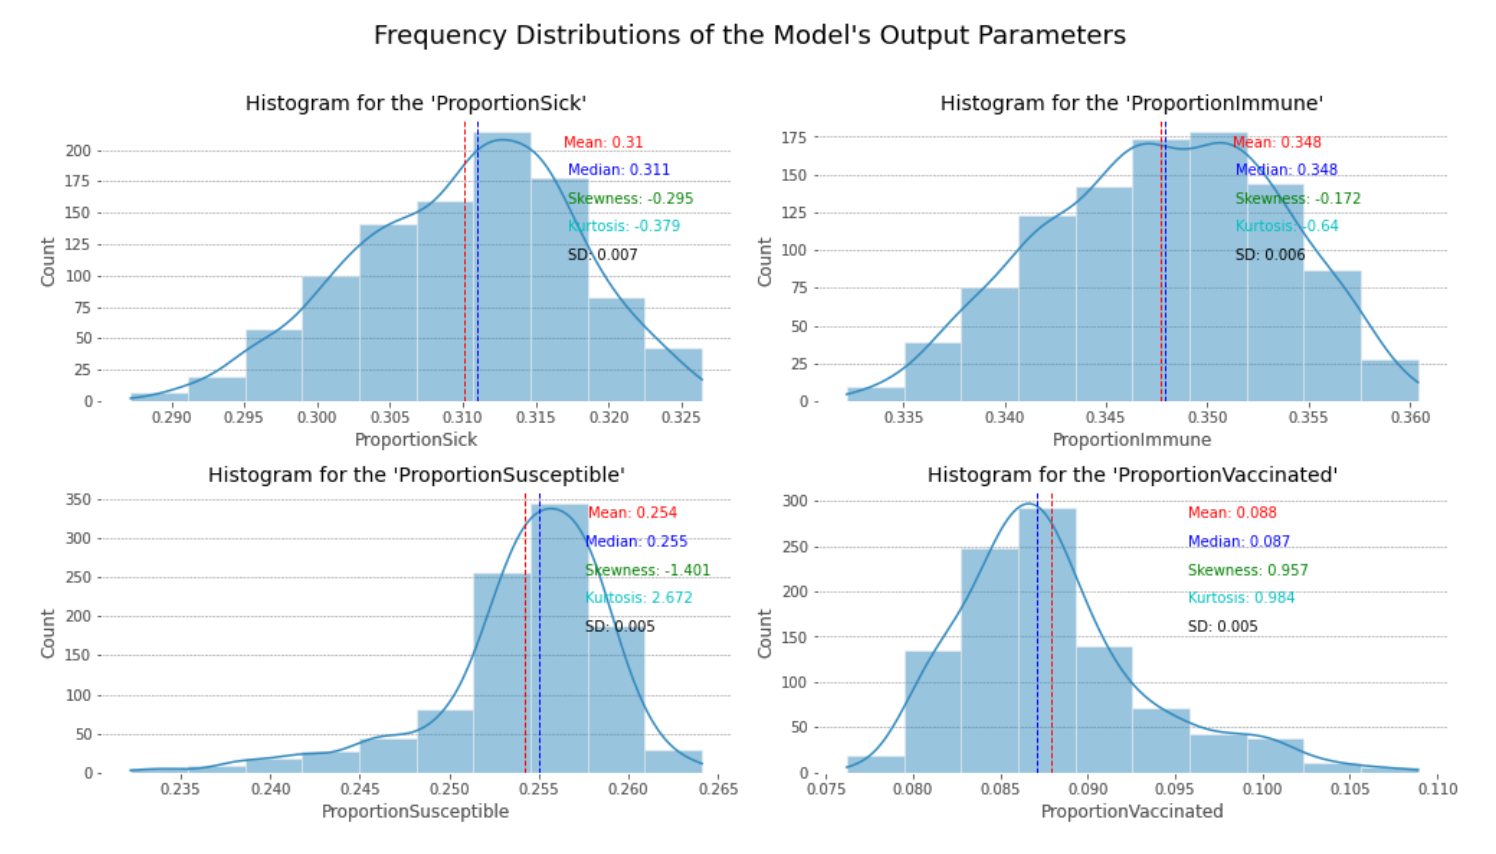
\includegraphics[width=0.49\linewidth]{../figures/histograms.png}
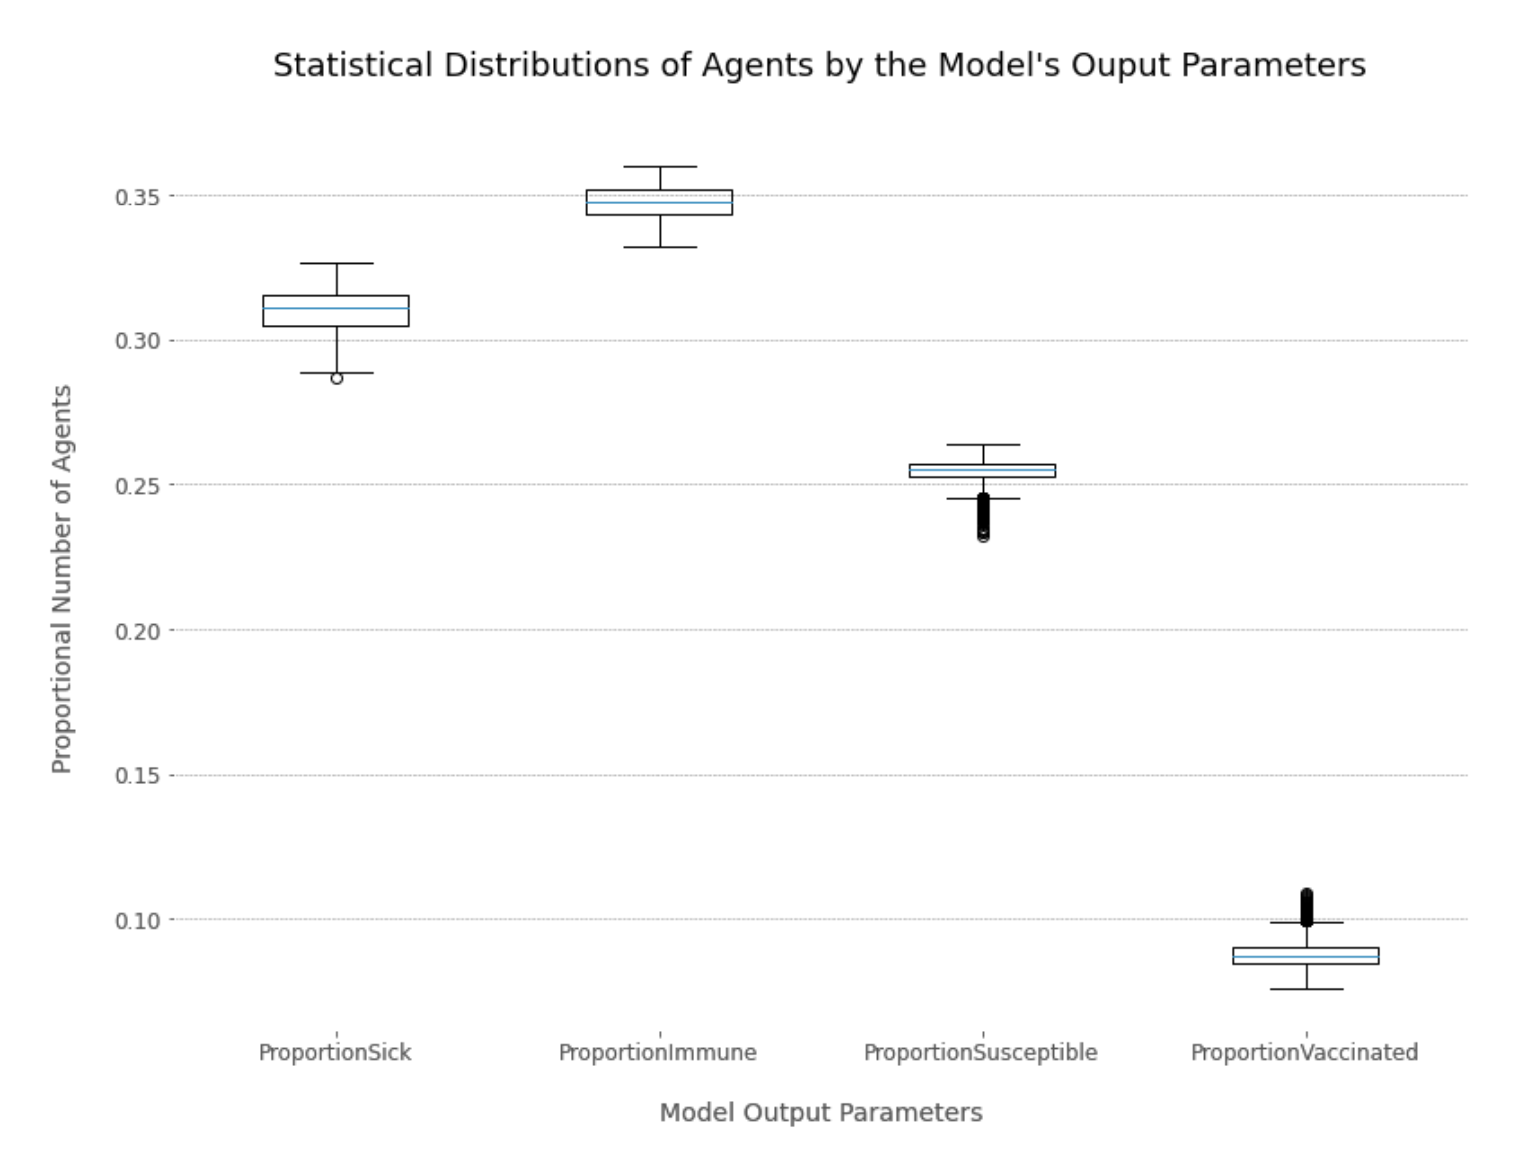
\includegraphics[width=0.49\linewidth]{../figures/agentTypeDistrib.png}

\bigskip
\bigskip

LHS sampling (10,000 points) to study statistical properties of model indicators: skewed distributions (Left), distributions of the proportion of agents in each state (Right)

}


\sframe{Grid exploration}{

%The total combination of the model's input parameters with predefined values is 81. The model run for each combination of the inputs is set to 125 times. This results in a total model run of 10,125 model runs, for a total execution time of 4 days and 5 hours.
% The box plots in Fig.~\ref{fig:boxplots} show statistical distributions of the ‘ProportionSick’, which are grouped by each input parameter value of the model. The range of each input parameter is indicated on the horizontal axis of the graphs. The first graph represents the grouped values of the ‘ProportionSick’ by the values of the ‘infectiousPeriod’. It indicates that a unit increase in the infectiousPeriod’ value increases the boxplot’s overall median and max values. The boxplots related to the ‘immunityPeriod’ and the ‘socialDistancingLevels’ show a marginal decrease in the median of the boxplots per unit increase. The last graph is related to the ‘vaccinationRate’, which indicates that a 0.0025 (0.25 \%) increase in the rate decreases the boxplot’s overall values. It indicates that vaccines have an apparent effect on successfully controlling the spread of diseases.
% The correlation matrix illustrated in Fig.~\ref{fig:correlations} displays the correlation between different model parameters. The ‘ProportionSick’ and the ‘infectiousPeriod’ appear to be highly correlated. According to the box plots shown in Figure 14, every unit increase in the ‘infectiousPeriod’ also increased the ‘ProportionSick’ values. The rest of the input parameters, including the ‘immunityPeriod’, ‘socialDistancingLevels’ and ‘vaccinationRate’ are negatively correlated with the ‘ProportionSick’ at different intensity levels.
%An OLS regression with the simulated data shows that the spread of infection mainly depends on the longevity of the infectious period. The longevity of the infectious period plays a vital role in disease transmission because a more extended infectious period allows an infected agent to interact with a more significant number of susceptible agents for an extended time. For example, an infected agent who is infectious for a single day is unlikely to infect a more significant number of susceptible agents than an infected agent who is infectious for a week. A more extended infectious period is, therefore, a dangerous factor that may rapidly increase the chances of infections, often creating a mass infection wave.

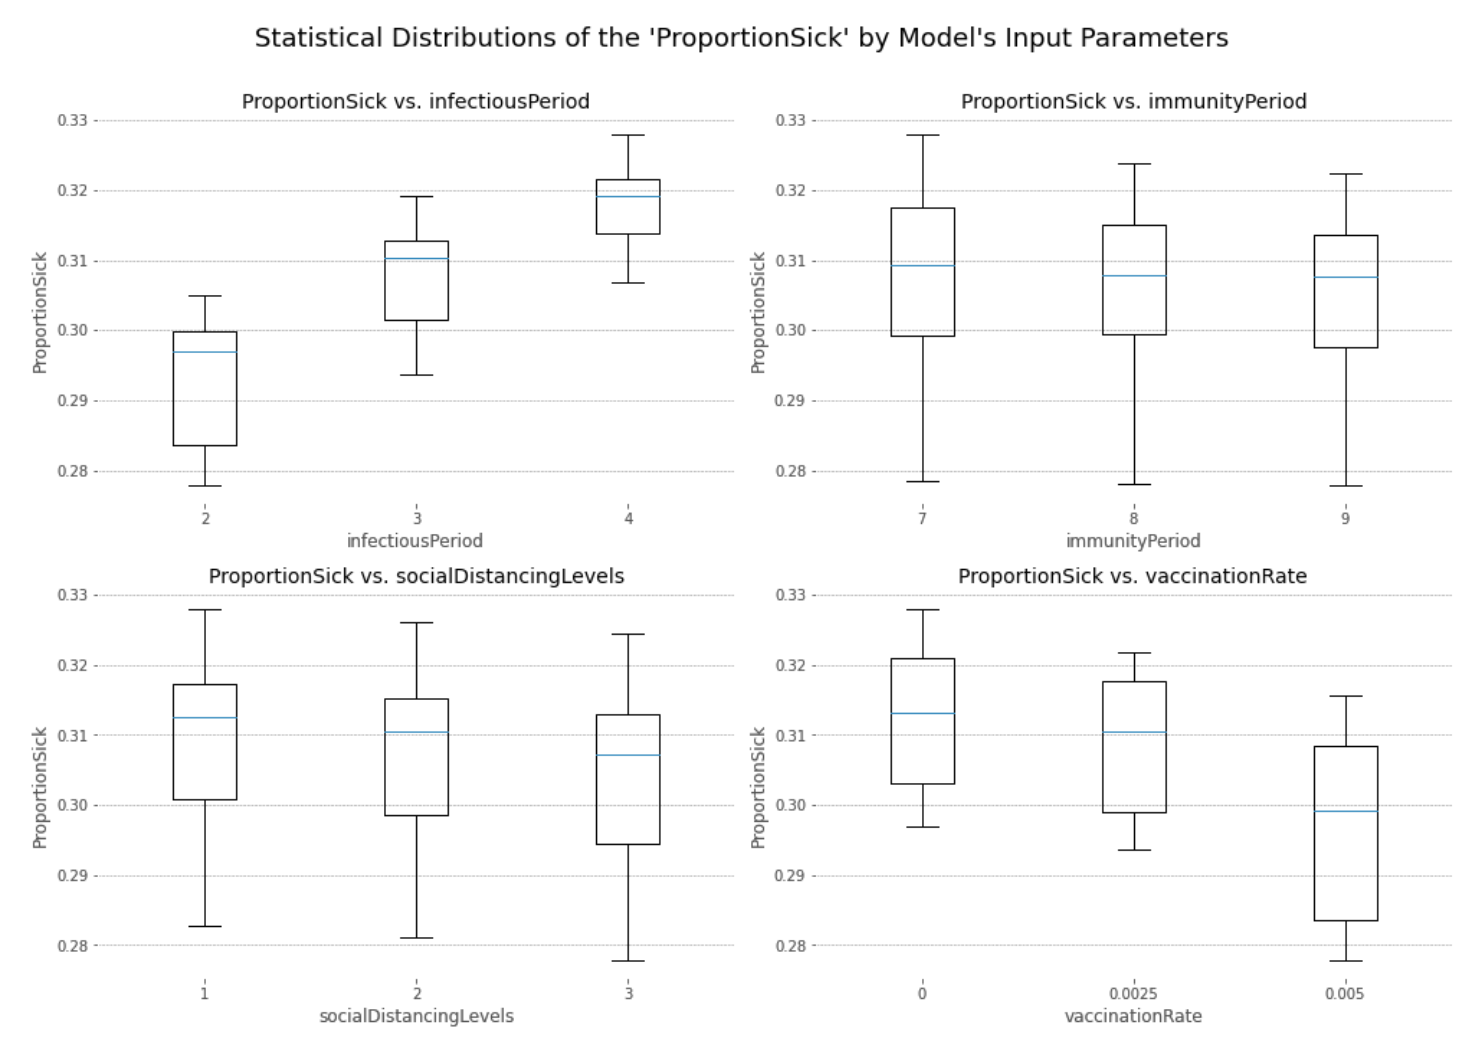
\includegraphics[width=0.49\linewidth]{../figures/boxplots.png}
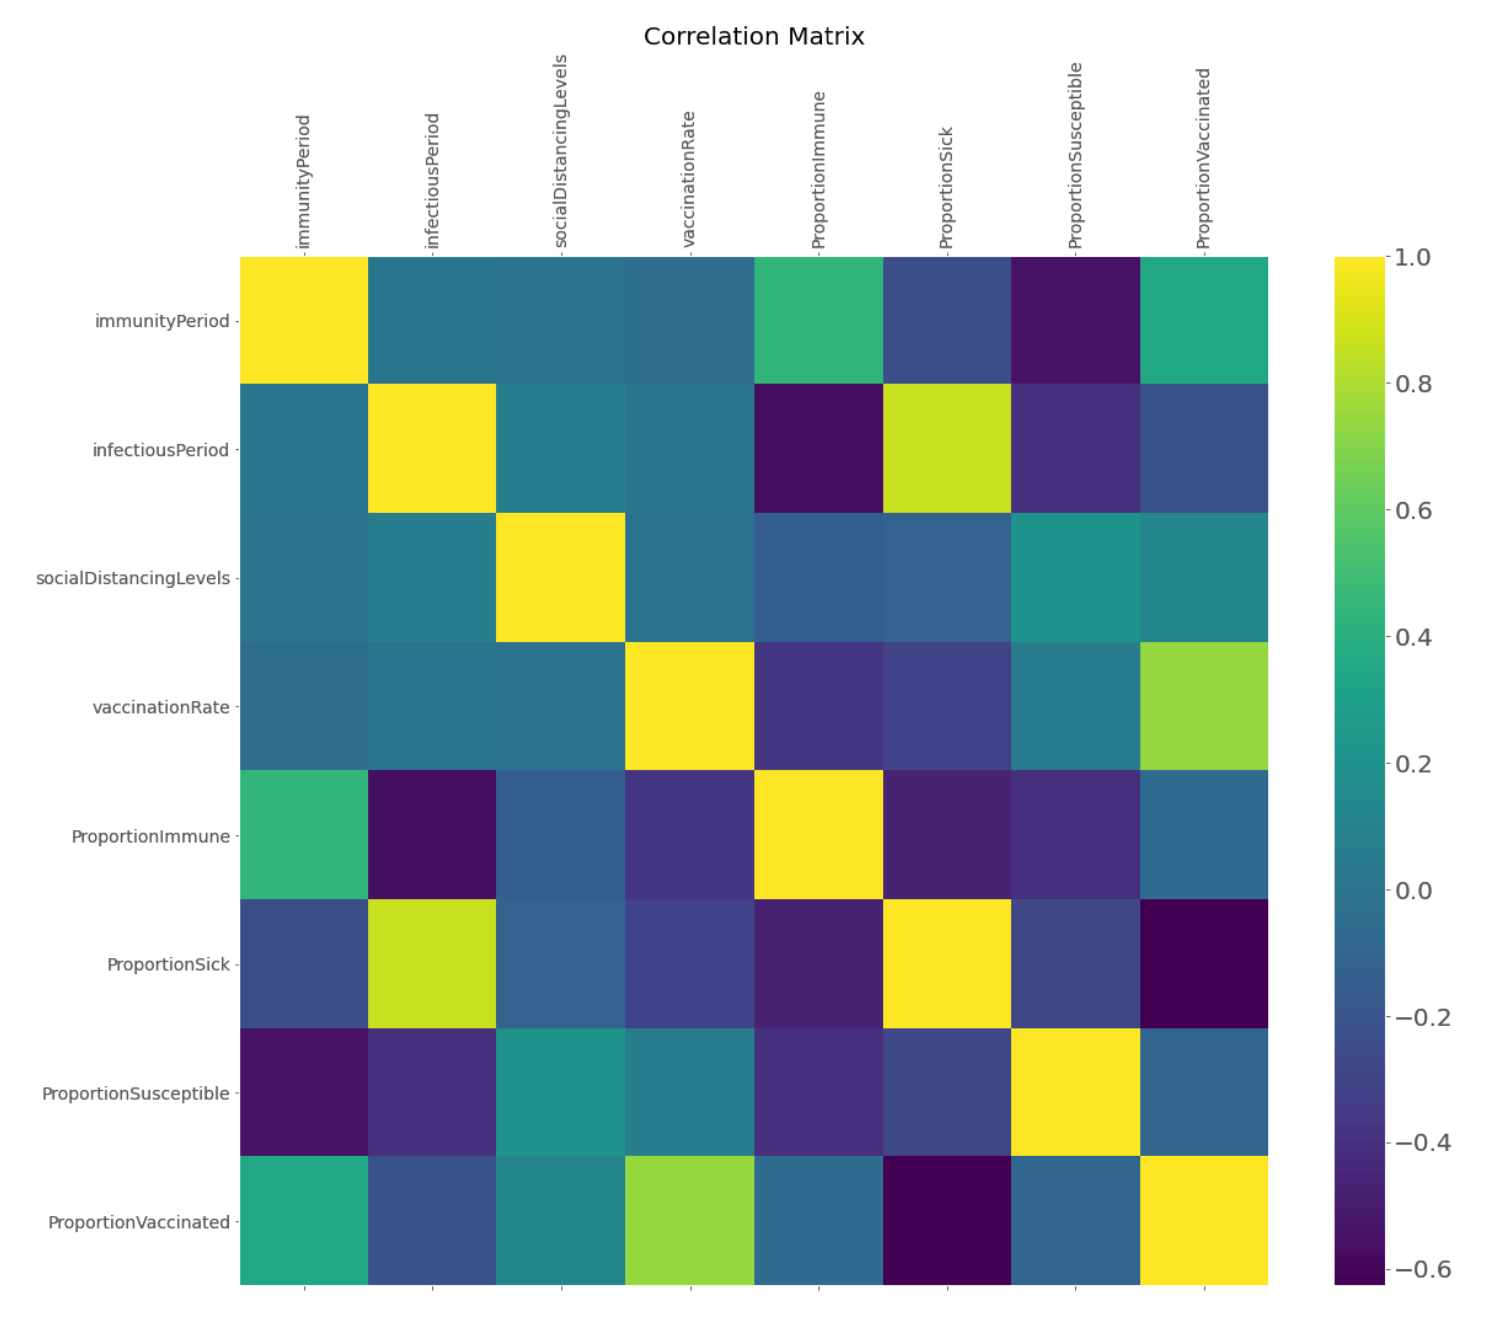
\includegraphics[width=0.49\linewidth]{../figures/correlations.png}

\bigskip
\bigskip

Grid exploration of 81 parameter points (125 stochastic repetitions for each): various amplitude of parameter influence (Left), confirmed with an OLS regression, and correlation matrix of model inputs and outputs (Right)

}

\sframe{Model surrogate}{

%Then, a random forest model is trained with the original data obtained by the LHS method during the first step of the analysis to forecast the proportional number of sick agents.
%In order to train the random forest model to predict the values of the ‘ProportionSick’, the original data is categorised into train, test, and validation data in the ratio of 7:1.5:1.5. Before fitting the model with the train data, various numbers of trees with their corresponding accuracy scores are calculated. Then, the hyperparameter for the model was optimised using the grid search method for a given set of estimator values, including 800, 900, 950, 1000 and 1050. As a result, 900 is the best value for optimising the random forest model. The random forest with the 900 decision trees was developed by fitting the training data to predict the values of the ‘ProportionSick’ and included the use of all four input parameters of the model.
%The predicted values of the 'ProportionSick' via the random forest are compared with the actual values in a table. The comparison between the statistical distributions of those two types of values is then visualised on a density plot.
%We obtain a MAE (how big of an error we can expect from the forecast on average) of 0.001, which implies that the average errors between the predicted and actual values are marginal; hence, the predictions are considered highly accurate. Moving on to the MAPE, the value of 0.363 indicates that, on average, the forecast is off by 0.363\%. This means that the accuracy of the forecast is as high as 99.637\%. Lastly, the value of the RMSE is also 0.001, which indicates that the difference between the predicted and actual values is marginal.
%The random forest model is furthermore useful to quantify the importance of the model’s input parameters, shown in Fig.~\ref{fig:randomForest}. The ‘infectiousPeriod’ is by far the most significant input parameter of the model, with a value of approximately 0.75. Followed by the ‘vaccinationRate’ with a value of slightly over 0.1. The ‘immunityPeriod’ and the ‘socialDistancingLevels’ had an importance rate below 0.1, which were not as significant as the previous two.

\begin{center}
   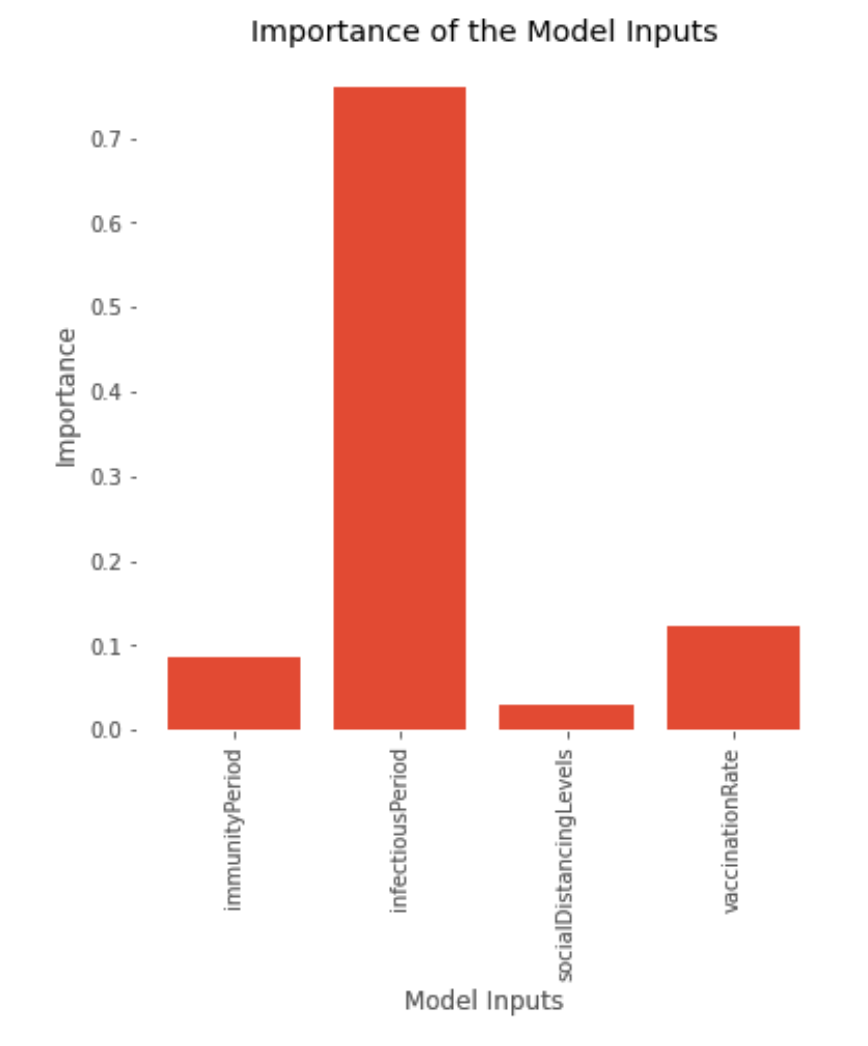
\includegraphics[width=0.45\linewidth]{../figures/randomForest.png}
\end{center}

\bigskip

Random forest model surrogate trained on LHS simulation data (performance: MAE=0.001): feature importance of input parameters.

}

\sframe{Global sensitivity analysis}{

%The previous results of parameter importance can be compared with an other method to quantify parameter's influence on indicators. The global sensitivity analysis method, introduced by \cite{saltelli2008global}, gives a broad summary of such an influence. In order to generate an accurate result for the sensitivity analysis, a total of 60,000 samples were run (25 days 7 hours of model runtime).
%The total-order indices shown above indicate that the ‘infectiousPeriod’ has the most significant impact on the values of the ‘ProportionSick’ followed by the ‘vaccinationRate’, ‘socialDistancingLevels’ and ‘immunityPeriod’ respectively. We find a very low effect of the immunity period on the proportion of sick and susceptible, meaning that uncertainties on this value will have a limited impact. The vaccination rate is also a critical input parameter of the model that plays a vital role in controlling the spread of diseases because the vaccine is a significant source of protective measures that can effectively stop viruses from transmitting one agent to another \cite{storlie2021quantifying}.

\begin{table}
\resizebox{\textwidth}{!}{
\begin{tabular}{|c|c|c|c|c|}
Outputs & infectiousPeriod & immunityPeriod & vaccinationRate & socialDistancingLevels\\
ProportionImmune & 0.72 & 0.333 & 0.665 & 0.7\\
ProportionSick & 0.692 & 0.09 & 0.365 & 0.143\\
ProportionVaccinated & 0.516 & 0.319 & 0.587 & 0.337\\
ProportionSusceptible & 0.341 & 0.066 & 0.92 & 0.277\\
\end{tabular}
}
\end{table}

\bigskip
\bigskip

Saltelli total order indices \cite{saltelli2008global} to quantify parameters' influence on model indicators.


}


\sframe{Multi-objective model optimisation}{

%In attempting to control the spread of epidemics, many problems involve multiple objectives which cannot simply be described as the more, the better or the lesser, the better; instead, each objective has an ideal target value, and the main goal is to reach the targeted value as close as possible. To optimise the values of the input parameters, we define two objectives that are expected to be minimised. Firstly, we expect the proportional number of sick agents to be optimised, which is directly linked to the main interest of our research question. Secondly, we expect the proportional number of vaccinated agents to be optimised. Vaccination is a primary preventive measure that plays a vital role in successfully controlling the spread of diseases and even has the potential to achieve herd immunity, while other measures such as social distancing can only slow down the process of disease spreading instead of stopping them \cite{bicher2022model}. However, vaccines are not always available for multiple reasons, and one of the possible reasons might be due to the high manufacturing and transportation costs \cite{plotkin2017complexity}. This is where people like decision- makers often face a dilemma because attempting to control epidemics usually costs money and the best option which they might have at this point is to find a good balance between the usage of vaccines, which does not go over the budget, and the proportional number of sick agents.
%The way to find the results that provide a good approximation of the Pareto frontier with acceptable trade-offs between the identified objectives is by using the NSGAII. The NSGAII is a commonly used type of multi-objective optimisation algorithm that consists of several unique characteristics. These characteristics include a fast non-dominated sorting, crowding distance assignment and sorting procedure \cite{deb2002fast}.
%The Pareto Front consisting of non-dominated solutions relative to the ‘ProportionSick’ and ‘ProportionVaccinated’ is drawn after running a total of 10,000 generations of the OpenMOLE implementation of the algorithm.
%3 days 19 hours = 3.79 days
%The Pareto Front shown in Fig.~\ref{fig:pareto} illustrates the optimal solution set of the ‘ProportionSick’ and the ‘vaccinationRate’ as two objectives. The value of the ‘ProportionSick’ appears to decrease rapidly as the value of the ‘vaccinationRate’ increases. The slope of the line is generally steep throughout the graph. Plus, the difference between the values of the ‘ProportionSick’ with and without the vaccination is clear. The non-linearity of the front is an interesting feature, witnessing the underlying complexity when exploring policy trade-offs.
%The Pareto Front, visualised in Fig.~\ref{fig:pareto2}, is formed with the optimal values of the ‘ProportionSick’ and the ‘socialDistancingLevels’ as two objectives. It indicates a clear sign of a decrease in the value of the ‘Proportionsick’ as the value of the ‘socialDistancingLevels’ increases. In some regions of the front, a quasi-vertical increase means that much control may be gained at a very low social cost, what has implications when finding the compromise between the epidemic impact and the social impact of lockdowns. The social distancing level is an essential input parameter that acts as a preventive measure against infectious diseases in our model. Social distancing must be implemented with care because if the intensity is too high, it prohibits necessary human interactions, which reduces the productivity rate, negatively impacting the economy in general \cite{deluca2020unequal}. Due to this, finding a good balance between the social distancing level and the proportional number of sick agents would be essential in ensuring a healthy economy while keeping the number of infected cases low.


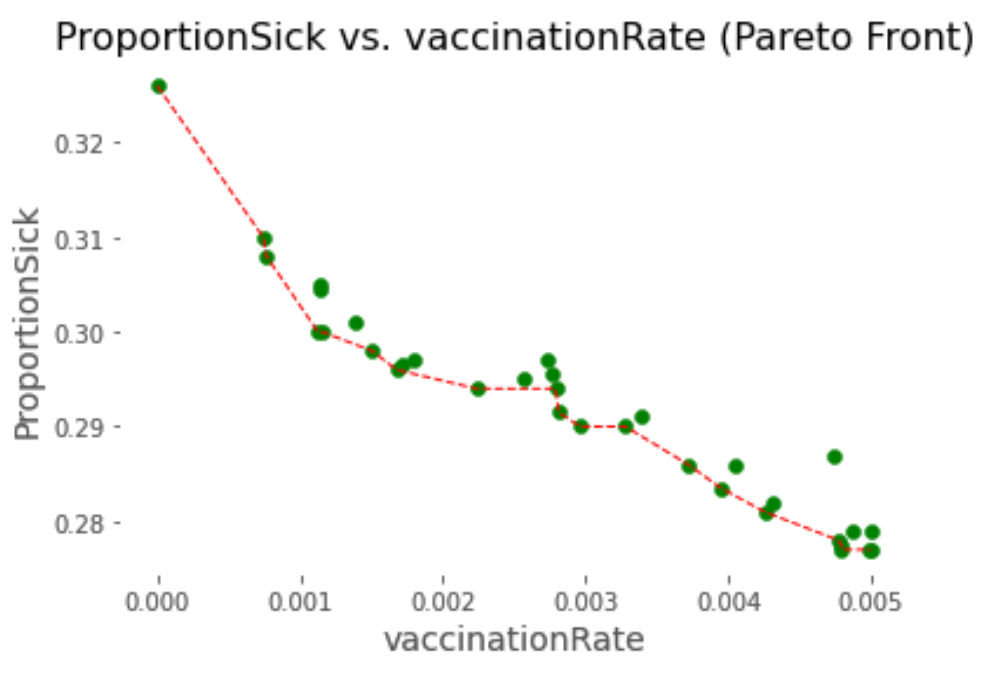
\includegraphics[width=0.49\linewidth]{../figures/pareto.png}
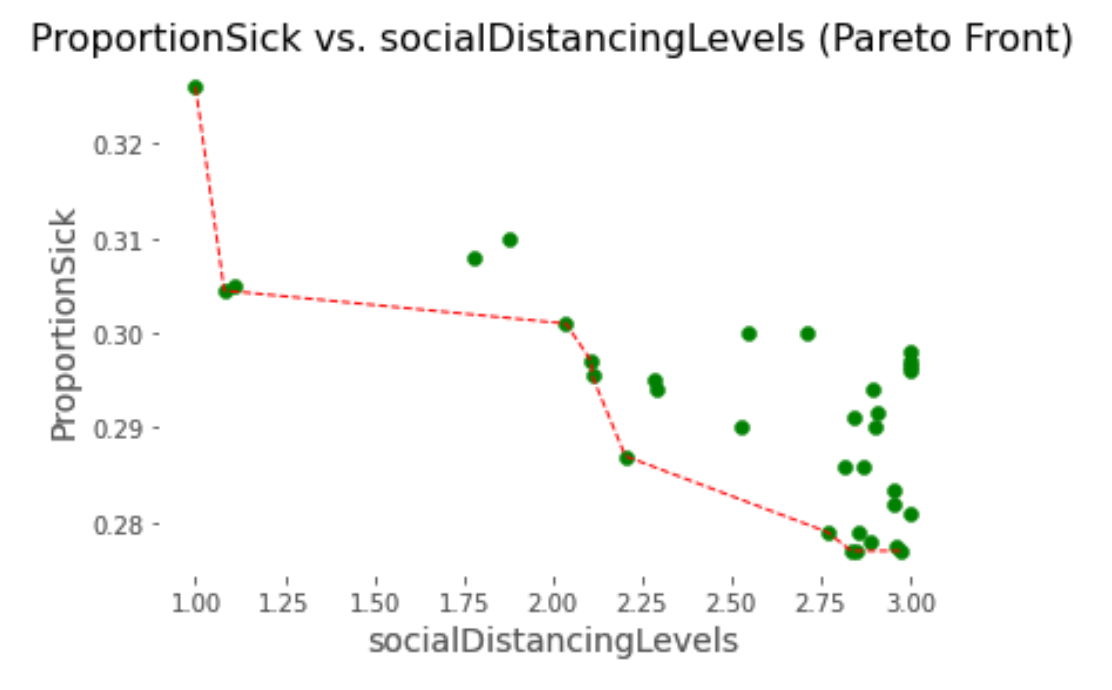
\includegraphics[width=0.49\linewidth]{../figures/pareto2.png}

\bigskip

NSGA2 bi-objective optimisation to find compromise points between disease burden and vaccination (cost): Pareto front of proportion of sick vs. social distancing levels (Left), and corresponding points on other objectives (Right).

}

\section{Discussion}


\sframe{Discussion}{

% The diverse numerical experiments, applying various model exploration and validation methods, provide useful policy insights in this stylised case. Thus, we suggest that our work is a proof-of-concept of how such systematic model exploration may hinder issues due to parameter uncertainty, or the lack of data, for similar epidemiological models.
%Some limitations of this work can be given. Firstly, the population size of the simulation had to be limited to a small number, mainly due to the expensive computational cost and time. In order to fasten the process, these executions have been distributed thanks to OpenMOLE, but the limitation in the level of detail and granularity is a recurring issue with ABMs. We still need to investigate if the trade-off chosen here is reasonable.
%The current number of input parameters is limited to only four parameters. However, there can be more numbers of input parameters introduced in our model to generate more dynamic results which can better reflect real-life situations. Furthermore, the current model can be constructed with extra compartments that can describe various states of an agent in the infection process. If compartments such as death or exposure are added to the model, the states of an agent can further be categorised into a more significant number of states and make the overall dynamics of disease transmission rather sophisticated for an advanced result \cite{reyne2022principles}. The model is also flexible in that it can add many more characteristics of agents, such as age, occupation, vaccination record and gender, which can be considered in the process of interaction and infection.
%As a future work, regarding the stylised parametrisation taken here for several aspects of model setup, a more advanced sensitivity analysis relaxing these parameters could be done. More particularly, quantifying the role of geography (transport geography, but also company size distribution and locations), is an interesting prospect, as new methods to achieve this have recently been developed \cite{raimbault2019space}.


$\rightarrow$ proof-of-concept of how model exploration and validation can compensate for parameter uncertainty and the lack of data

\medskip

$\rightarrow$ open question: transfer to policy scenarios, which practical validated insights from such hybrid approaches

\medskip

$\rightarrow$ model can be refined in several ways (e.g. agent states, more characteristics)

\medskip

$\rightarrow$ sensitivity to geography and to the company setup \cite{raimbault2019space} to be explored


}



\sframe{Conclusion}{

% This study proposed various model assessment methods to explore results obtained with a stylised ABM we introduced, based on the SIRV compartmental model to study the spread of diseases. Through the model, this study analysed the impacts of the pre-defined input parameters, which included the infectious period, immunity period, daily vaccination rate and social distancing level on the spread of infectious diseases. We provide thus a proof-of-concept of how model exploration and validation methods can be a powerful tool to design and optimise health policies.



\justify

$\rightarrow$ a simple and stylised ABM based on SIRV accounting for geography and commuting

\medskip

$\rightarrow$ systematic exploration and sensitivity analysis: prospects on how to design and optimise health policies in cases where data or modelling resources are lacking


\bigskip
\bigskip



\textbf{Open repository}


\url{https://github.com/henry-kang-7/CASA0004} 




}






%%%%%%%%%%%%%%%%%%%%%
\begin{frame}[allowframebreaks]
\frametitle{References}
\bibliographystyle{apalike}
\bibliography{../biblio}
\end{frame}
%%%%%%%%%%%%%%%%%%%%%%%%%%%%










\end{document}





